\subsection{Quaternion}
\[
    \bm{q} = \begin{bmatrix}
        q_0 \\
        q_1 \\
        q_2 \\
        q_3
    \end{bmatrix}
\]
\[
    \bm{q} = \begin{bmatrix}
        \cos(\dfrac{\psi}{2})\cos(\dfrac{\theta}{2})\cos(\dfrac{\phi}{2}) + \sin(\dfrac{\psi}{2})\sin(\dfrac{\theta}{2})\sin(\dfrac{\phi}{2}) \\[2em]
        \cos(\dfrac{\psi}{2})\cos(\dfrac{\theta}{2})\sin(\dfrac{\phi}{2}) - \sin(\dfrac{\psi}{2})\sin(\dfrac{\theta}{2})\cos(\dfrac{\phi}{2}) \\[2em]
        \cos(\dfrac{\psi}{2})\sin(\dfrac{\theta}{2})\cos(\dfrac{\phi}{2}) + \sin(\dfrac{\psi}{2})\cos(\dfrac{\theta}{2})\sin(\dfrac{\phi}{2}) \\[2em]
        \sin(\dfrac{\psi}{2})\cos(\dfrac{\theta}{2})\cos(\dfrac{\phi}{2}) - \cos(\dfrac{\psi}{2})\sin(\dfrac{\theta}{2})\sin(\dfrac{\phi}{2})
    \end{bmatrix}
\]
\[
    \dot{\bm{q}} = \dfrac{1}{2}\begin{bmatrix}
        0 & -p & -q & -r \\
        p & 0 & r & -q \\
        q & -r & 0 & p \\
        r & q & -p & 0
    \end{bmatrix} \bm{q}
\]
\[
    \bm{R} = \begin{bmatrix}
        q_0^2 + q_1^2 - q_2^2 - q_3^2 & 2(q_1q_2 - q_0q_3) & 2(q_1q_3 + q_0q_2) \\
        2(q_1q_2 + q_0q_3) & q_0^2 - q_1^2 + q_2^2 - q_3^2 & 2(q_2q_3 - q_0q_1) \\
        2(q_1q_3 - q_0q_2) & 2(q_2q_3 + q_0q_1) & q_0^2 - q_1^2 - q_2^2 + q_3^2
    \end{bmatrix}
    \]

    \begin{figure}[H]
        \centering
        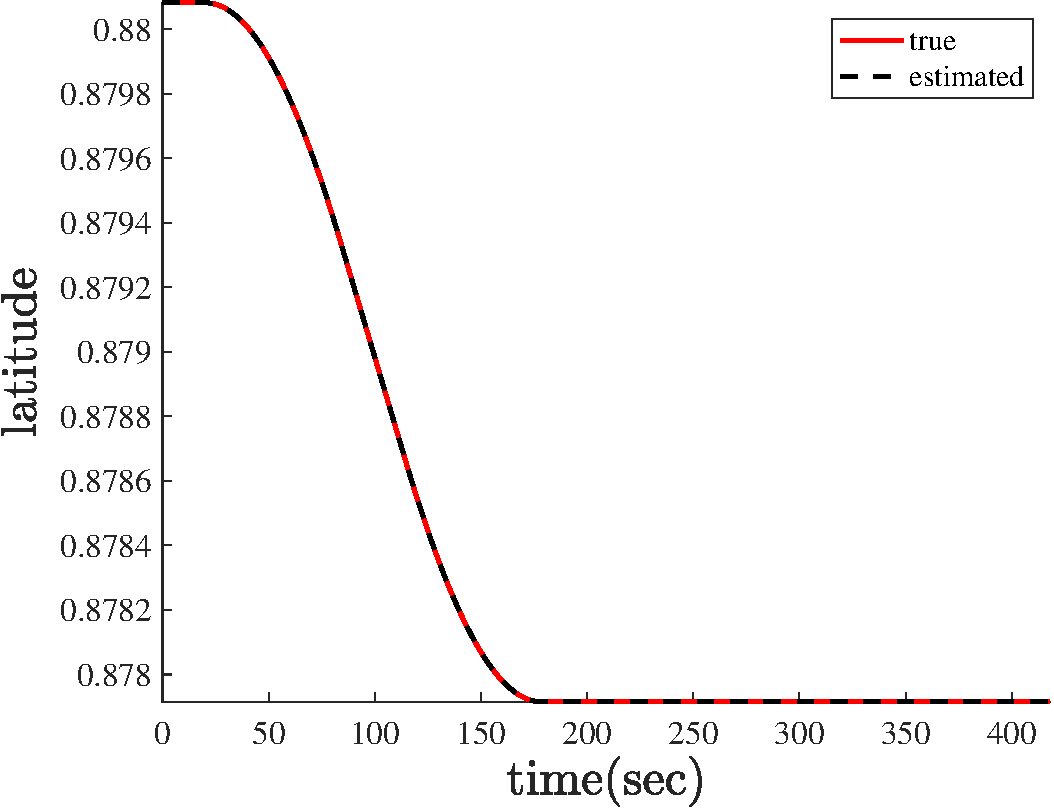
\includegraphics[width=0.7\textwidth]{../Figure/Q5/latitude_q}
        \caption{Latitude}
    \end{figure}
    \begin{figure}[H]
        \centering
        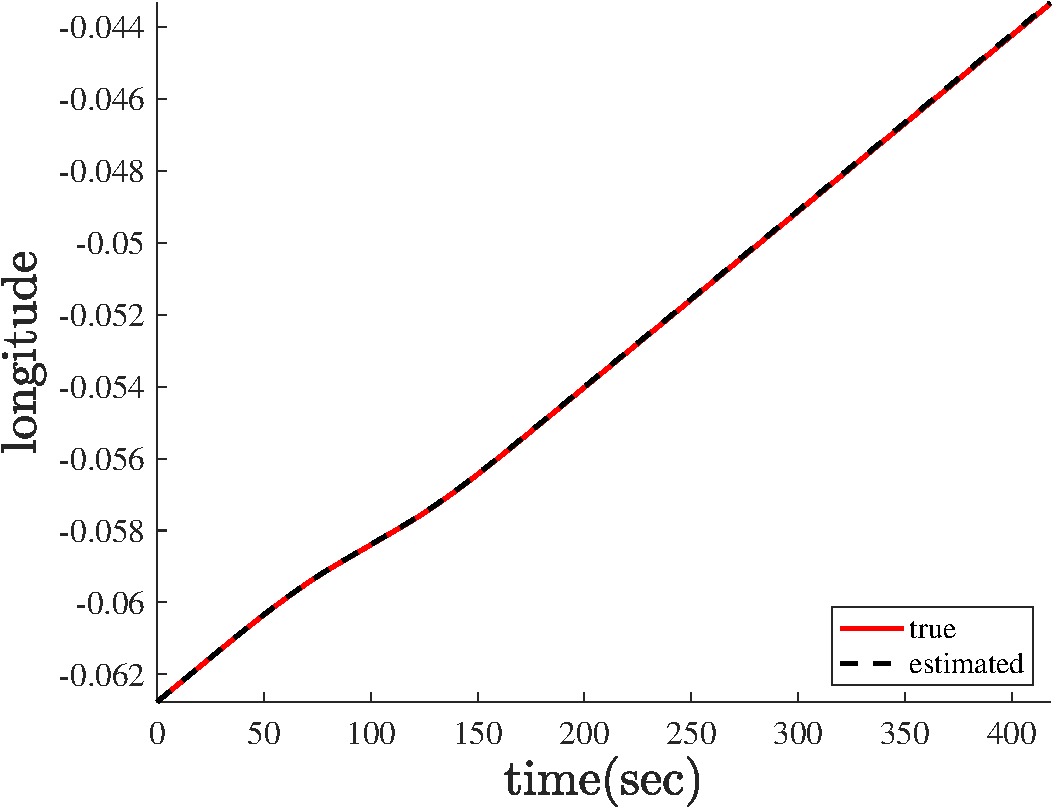
\includegraphics[width=0.7\textwidth]{../Figure/Q5/longitude_q}
        \caption{Longitude}
    \end{figure}
    \begin{figure}[H]
        \centering
        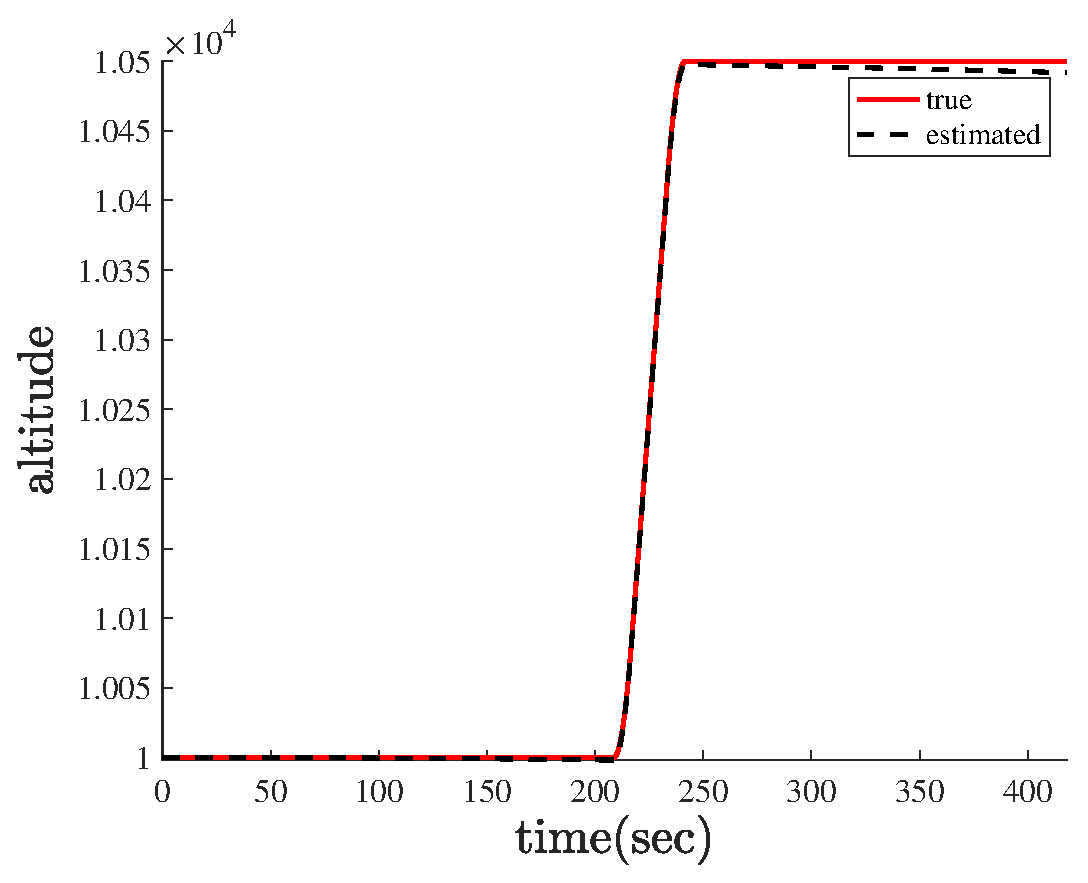
\includegraphics[width=0.7\textwidth]{../Figure/Q5/altitude_q}
        \caption{Altitude}
    \end{figure}
    \begin{figure}[H]
        \centering
        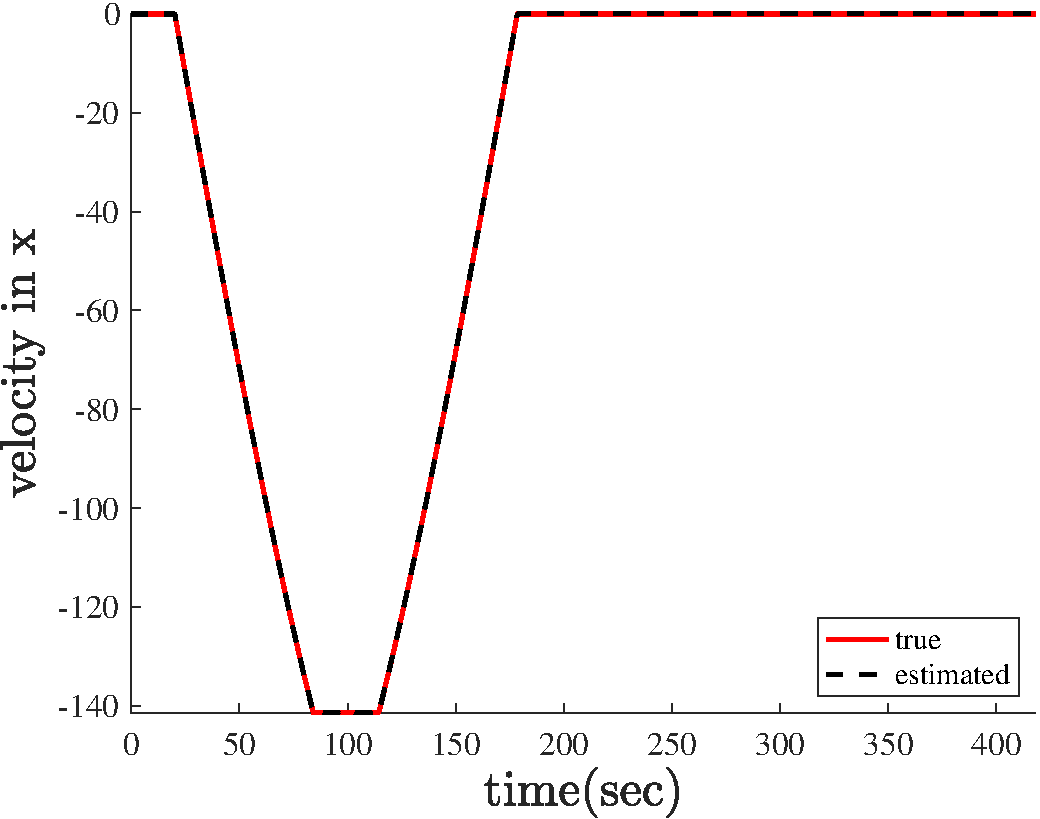
\includegraphics[width=0.7\textwidth]{../Figure/Q5/velocity_x_q}
        \caption{Velocity in x direction}
    \end{figure}
    \begin{figure}[H]
        \centering
        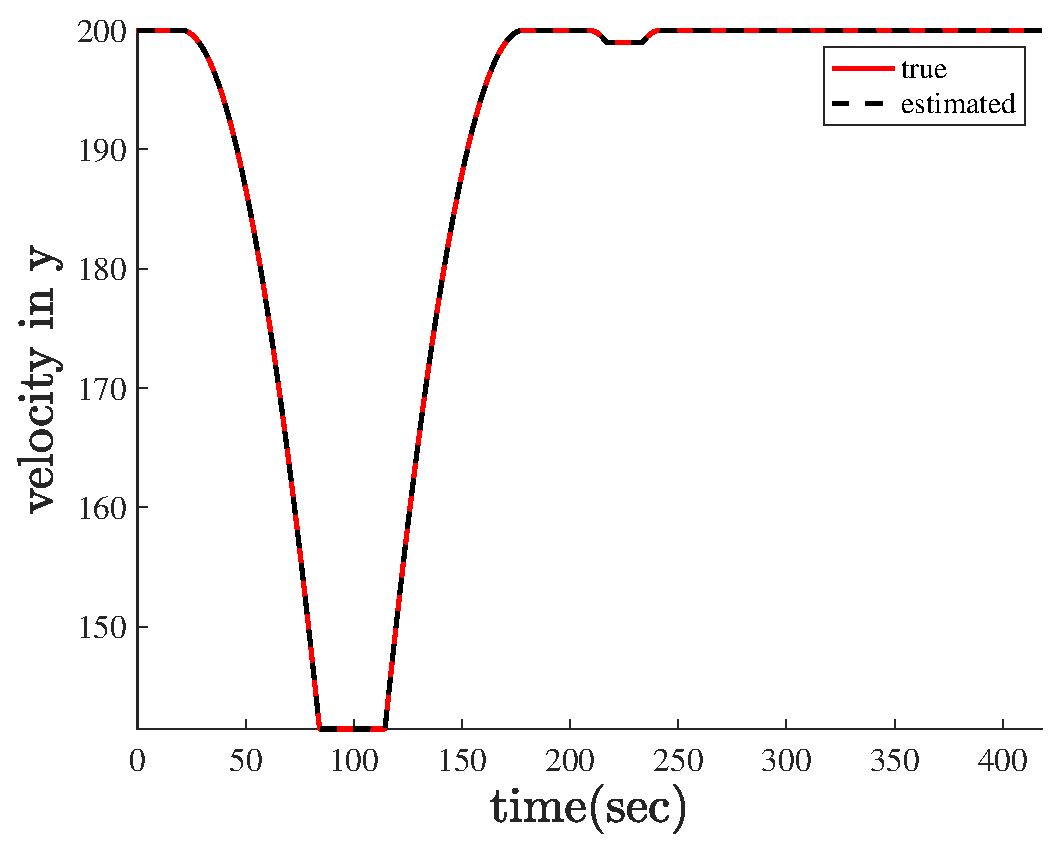
\includegraphics[width=0.7\textwidth]{../Figure/Q5/velocity_y_q}
        \caption{Velocity in y direction}
    \end{figure}
    \begin{figure}[H]
        \centering
        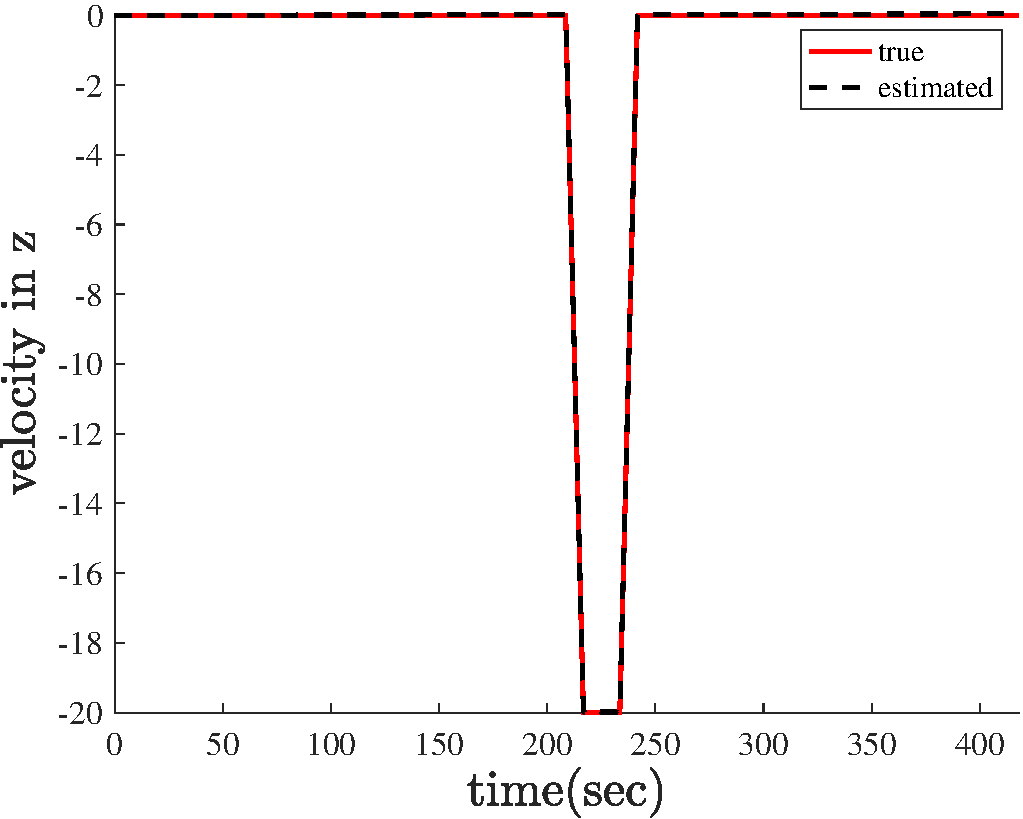
\includegraphics[width=0.7\textwidth]{../Figure/Q5/velocity_z_q}
        \caption{Velocity in z direction}
    \end{figure}
    
    \begin{figure}
        \centering
        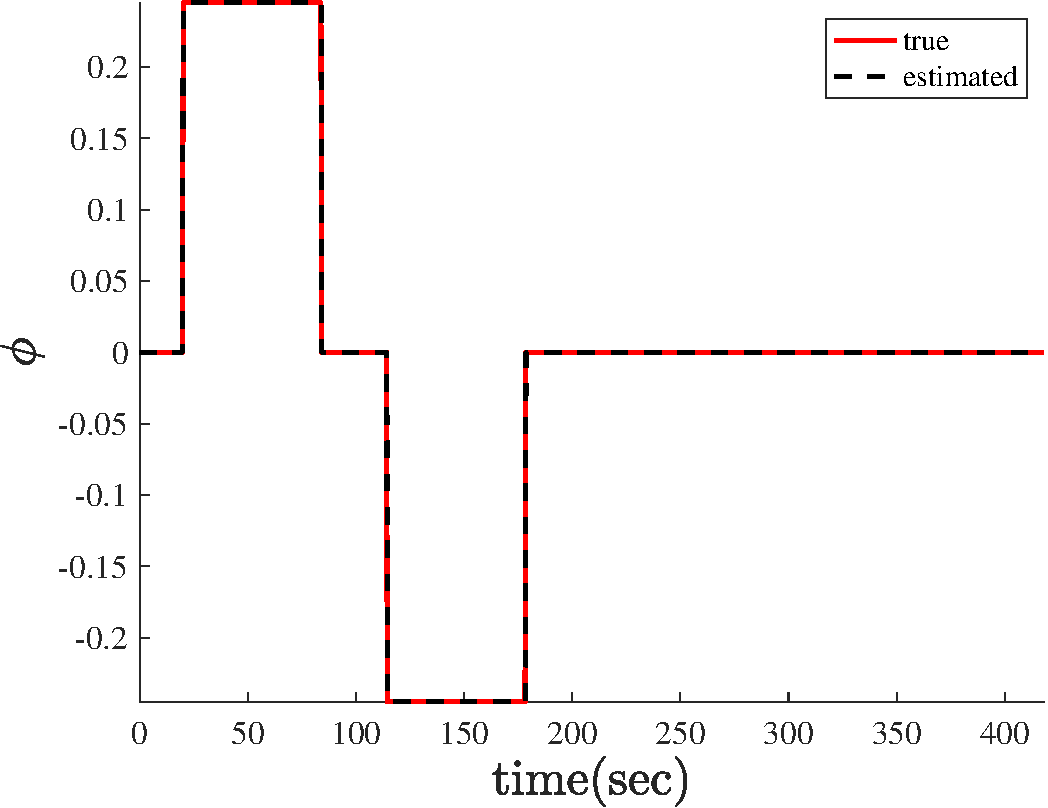
\includegraphics[width=0.7\textwidth]{../Figure/Q5/phi_q}
        \caption{Roll}
    \end{figure}
    \begin{figure}
        \centering
        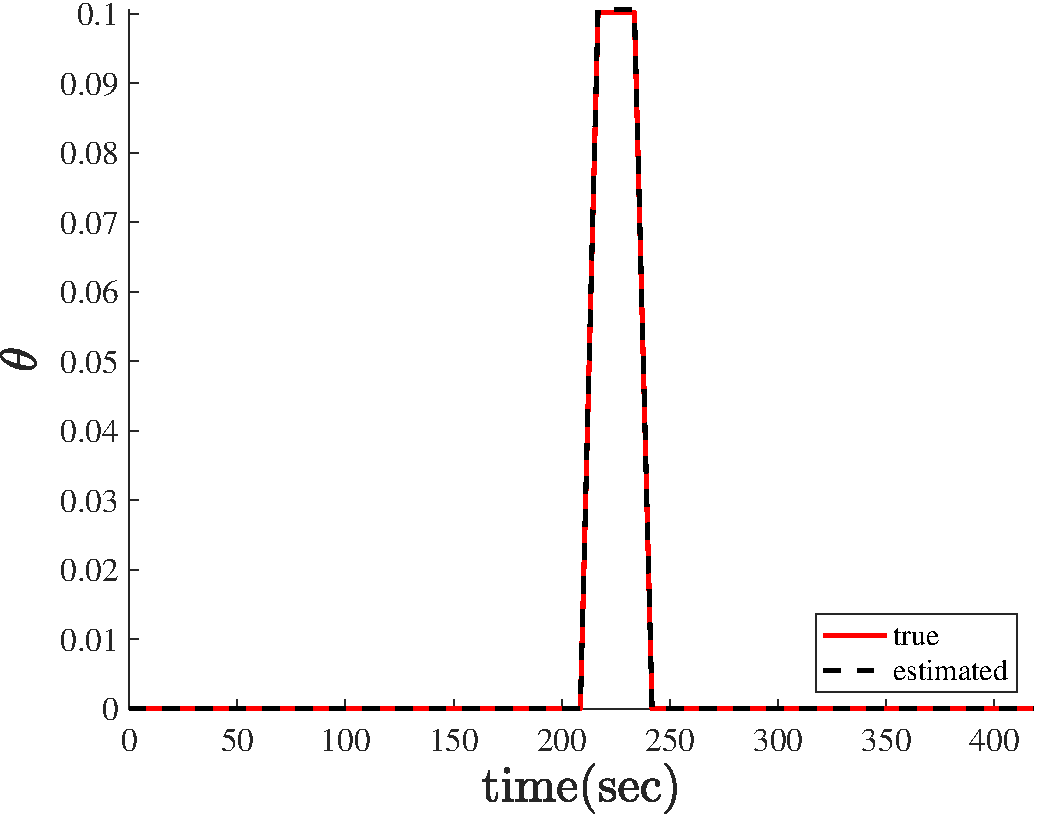
\includegraphics[width=0.7\textwidth]{../Figure/Q5/theta_q}
        \caption{Pitch}
    \end{figure}
    \begin{figure}
        \centering
        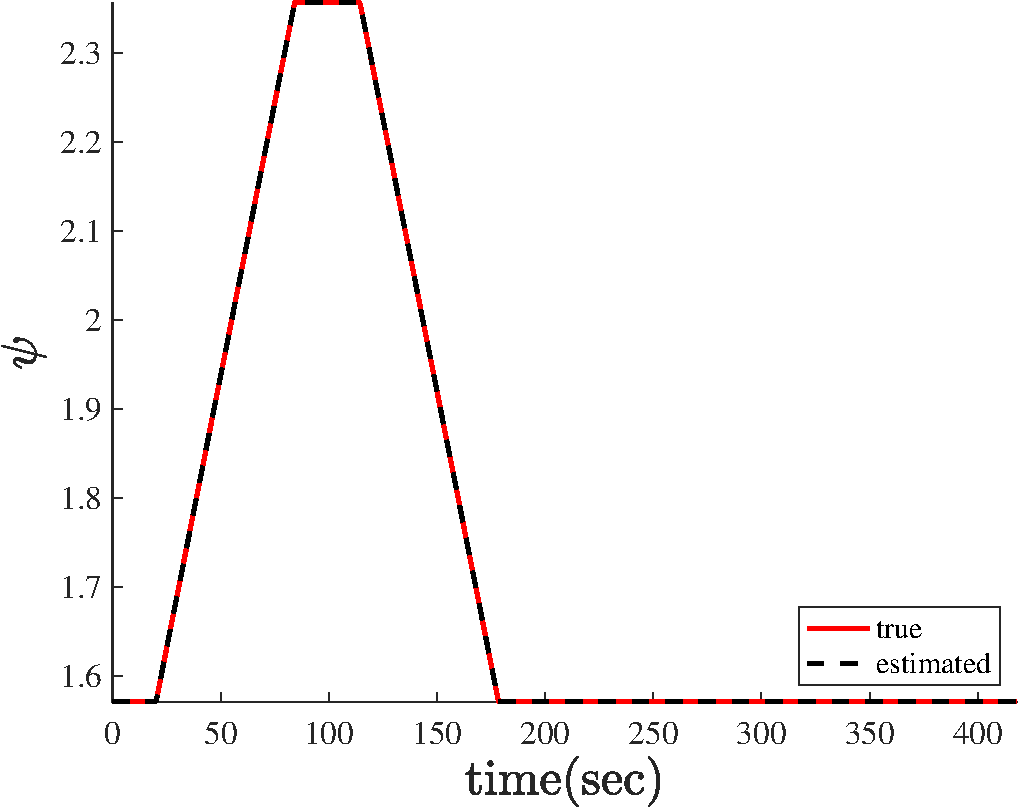
\includegraphics[width=0.7\textwidth]{../Figure/Q5/psi_q}
        \caption{Yaw}
    \end{figure}
